% Options for packages loaded elsewhere
\PassOptionsToPackage{unicode}{hyperref}
\PassOptionsToPackage{hyphens}{url}
%
\documentclass[
  11pt,
]{article}
\usepackage{amsmath,amssymb}
\usepackage{iftex}
\ifPDFTeX
  \usepackage[T1]{fontenc}
  \usepackage[utf8]{inputenc}
  \usepackage{textcomp} % provide euro and other symbols
\else % if luatex or xetex
  \usepackage{unicode-math} % this also loads fontspec
  \defaultfontfeatures{Scale=MatchLowercase}
  \defaultfontfeatures[\rmfamily]{Ligatures=TeX,Scale=1}
\fi
\usepackage{lmodern}
\ifPDFTeX\else
  % xetex/luatex font selection
\fi
% Use upquote if available, for straight quotes in verbatim environments
\IfFileExists{upquote.sty}{\usepackage{upquote}}{}
\IfFileExists{microtype.sty}{% use microtype if available
  \usepackage[]{microtype}
  \UseMicrotypeSet[protrusion]{basicmath} % disable protrusion for tt fonts
}{}
\makeatletter
\@ifundefined{KOMAClassName}{% if non-KOMA class
  \IfFileExists{parskip.sty}{%
    \usepackage{parskip}
  }{% else
    \setlength{\parindent}{0pt}
    \setlength{\parskip}{6pt plus 2pt minus 1pt}}
}{% if KOMA class
  \KOMAoptions{parskip=half}}
\makeatother
\usepackage{xcolor}
\usepackage[margin=1in]{geometry}
\usepackage{longtable,booktabs,array}
\usepackage{calc} % for calculating minipage widths
% Correct order of tables after \paragraph or \subparagraph
\usepackage{etoolbox}
\makeatletter
\patchcmd\longtable{\par}{\if@noskipsec\mbox{}\fi\par}{}{}
\makeatother
% Allow footnotes in longtable head/foot
\IfFileExists{footnotehyper.sty}{\usepackage{footnotehyper}}{\usepackage{footnote}}
\makesavenoteenv{longtable}
\usepackage{graphicx}
\makeatletter
\def\maxwidth{\ifdim\Gin@nat@width>\linewidth\linewidth\else\Gin@nat@width\fi}
\def\maxheight{\ifdim\Gin@nat@height>\textheight\textheight\else\Gin@nat@height\fi}
\makeatother
% Scale images if necessary, so that they will not overflow the page
% margins by default, and it is still possible to overwrite the defaults
% using explicit options in \includegraphics[width, height, ...]{}
\setkeys{Gin}{width=\maxwidth,height=\maxheight,keepaspectratio}
% Set default figure placement to htbp
\makeatletter
\def\fps@figure{htbp}
\makeatother
\setlength{\emergencystretch}{3em} % prevent overfull lines
\providecommand{\tightlist}{%
  \setlength{\itemsep}{0pt}\setlength{\parskip}{0pt}}
\setcounter{secnumdepth}{5}
\newlength{\cslhangindent}
\setlength{\cslhangindent}{1.5em}
\newlength{\csllabelwidth}
\setlength{\csllabelwidth}{3em}
\newlength{\cslentryspacingunit} % times entry-spacing
\setlength{\cslentryspacingunit}{\parskip}
\newenvironment{CSLReferences}[2] % #1 hanging-ident, #2 entry spacing
 {% don't indent paragraphs
  \setlength{\parindent}{0pt}
  % turn on hanging indent if param 1 is 1
  \ifodd #1
  \let\oldpar\par
  \def\par{\hangindent=\cslhangindent\oldpar}
  \fi
  % set entry spacing
  \setlength{\parskip}{#2\cslentryspacingunit}
 }%
 {}
\usepackage{calc}
\newcommand{\CSLBlock}[1]{#1\hfill\break}
\newcommand{\CSLLeftMargin}[1]{\parbox[t]{\csllabelwidth}{#1}}
\newcommand{\CSLRightInline}[1]{\parbox[t]{\linewidth - \csllabelwidth}{#1}\break}
\newcommand{\CSLIndent}[1]{\hspace{\cslhangindent}#1}
\usepackage{booktabs}
\usepackage{bm}
\usepackage{extarrows}
\setlength{\columnsep}{20pt}
\usepackage{booktabs}
\usepackage{longtable}
\usepackage{array}
\usepackage{multirow}
\usepackage{wrapfig}
\usepackage{float}
\usepackage{colortbl}
\usepackage{pdflscape}
\usepackage{tabu}
\usepackage{threeparttable}
\usepackage{threeparttablex}
\usepackage[normalem]{ulem}
\usepackage{makecell}
\usepackage{xcolor}
\ifLuaTeX
  \usepackage{selnolig}  % disable illegal ligatures
\fi
\IfFileExists{bookmark.sty}{\usepackage{bookmark}}{\usepackage{hyperref}}
\IfFileExists{xurl.sty}{\usepackage{xurl}}{} % add URL line breaks if available
\urlstyle{same}
\hypersetup{
  pdftitle={STAT 679 Final Project Report},
  pdfauthor={Xiaoyang Wang; Ziang Zeng},
  hidelinks,
  pdfcreator={LaTeX via pandoc}}

\title{\textbf{STAT 679 Final Project Report}}
\author{Xiaoyang Wang \and Ziang Zeng}
\date{}

\begin{document}
\maketitle

\hypertarget{astronomical-challange}{%
\section{Astronomical Challange}\label{astronomical-challange}}

Our project focuses on classifying celestial objects into stars, galaxies or quasars using their spectral characteristics. With the advancement of astronomical technology, we can obtain a large amount of data, including images and spectral information, from telescopes and large-scale photometry.

The central question of our project is: ``How can we effectively use image and spectral data to accurately classify different types of stellar objects?'' There are many machine learning methods and statistical models can be applied to classify the celestial objects. However, different methods and models performs differently on same data, ``All models are wrong but some are useful.'' Can we find a more ``useful'' model through combining several models together? Our solution is the voting classifier.

\hypertarget{data}{%
\section{Data}\label{data}}

We plan to work with the astronomy data set containing three types of data: images of the celestial objects, images of the spectrum, and the metadata of the objects. The first row in Figure \ref{fig:data_images} displays images of a galaxy, a star, and a quasar, from left to right, respectively. The second row in Figure \ref{fig:data_images} displays images of the spectrum of a galaxy, a star, and a quasar, from left to right, respectively. Table \ref{tab:metadata} provides explanations of the variables within the metadata.

\begin{figure}
\centering
\begin{minipage}{0.8\textwidth}
\centering
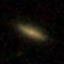
\includegraphics[width=\linewidth]{./data/GALAXY/GALAXY_1.jpg}\hfill
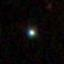
\includegraphics[width=\linewidth]{./data/STAR/STAR_1.jpg}\hfill
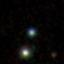
\includegraphics[width=\linewidth]{./data/QSO/QSO_1.jpg}

\end{minipage}
\end{figure}

\begin{figure}
\centering
\begin{minipage}{\textwidth}
\centering
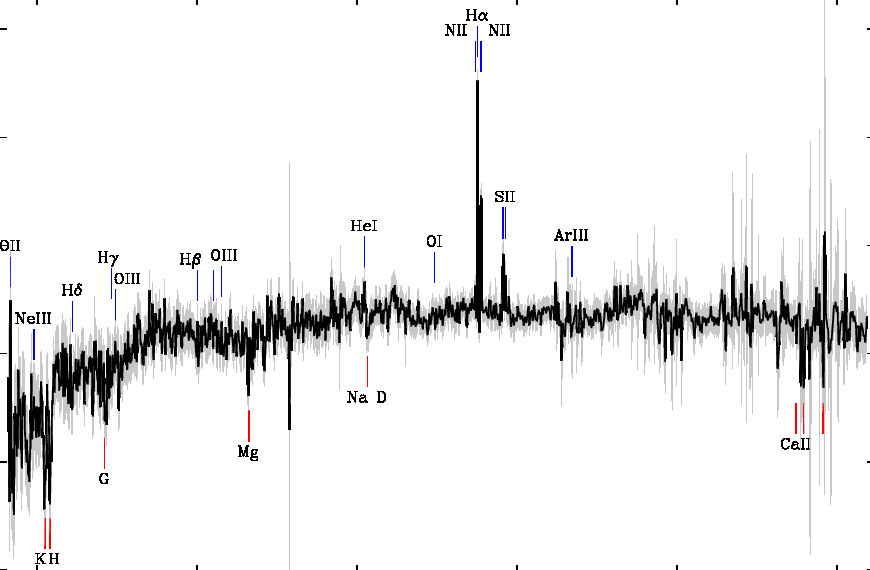
\includegraphics[width=0.3\linewidth]{./data/GALAXY_spec/GALAXY_spectrum_1.jpg}\hfill
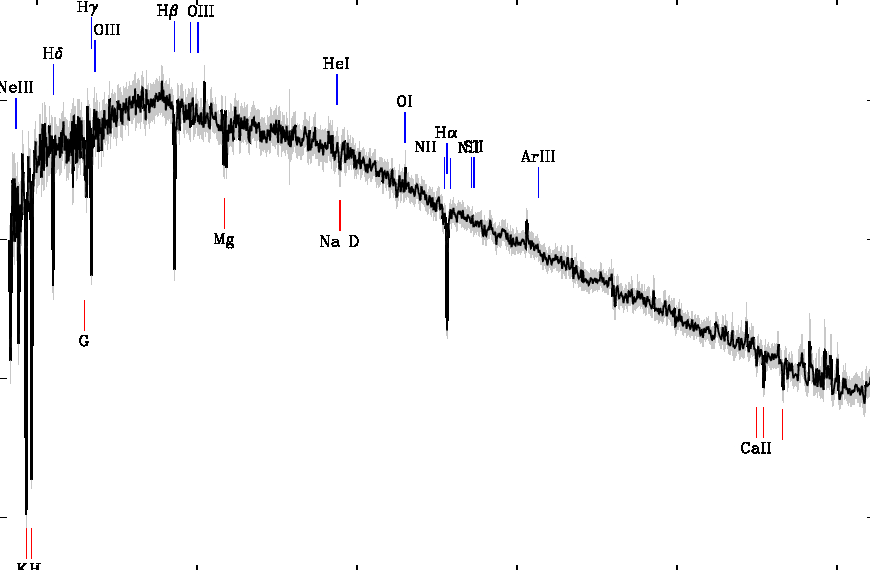
\includegraphics[width=0.3\linewidth]{./data/STAR_spec/STAR_spectrum_1.jpg}\hfill
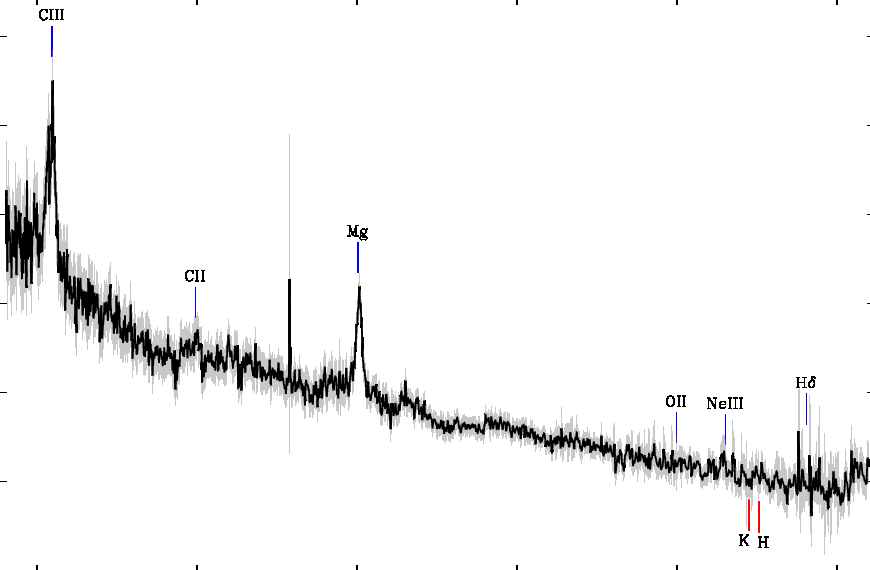
\includegraphics[width=0.3\linewidth]{./data/QSO_spec/QSO_spectrum_1.jpg}
\caption{Images of Celestial Objects and Corresponding Spectrum Images.}
\label{fig:data_images}
\end{minipage}
\end{figure}

They can be found in this \href{https://github.com/siriuszza/stat679final/tree/main/data}{\textcolor{blue}{link}}. All the data is obtained from \url{https://www.sdss.org}. Moreover, the distribution of classes of the celestial objects is 33333 samples each, which is selected from the website to make sure the dataset is balanced. Moreover, we encode the class with the following mapping: Galaxy \textasciitilde{} 0, Quasar \textasciitilde{} 1, Star \textasciitilde{} 2.

\hypertarget{exploratory-data-analysis}{%
\section{Exploratory Data Analysis}\label{exploratory-data-analysis}}

First, we will conduct exploratory data analysis on our dataset to better understand it and to find any possible errors. Figure \ref{fig:boxplot} shows the distribution of variables that are meaningful for classification. We can see that the means of all variables across different classes are quite different. Moreover, there are no significant outliers.

\begin{figure}
\centering
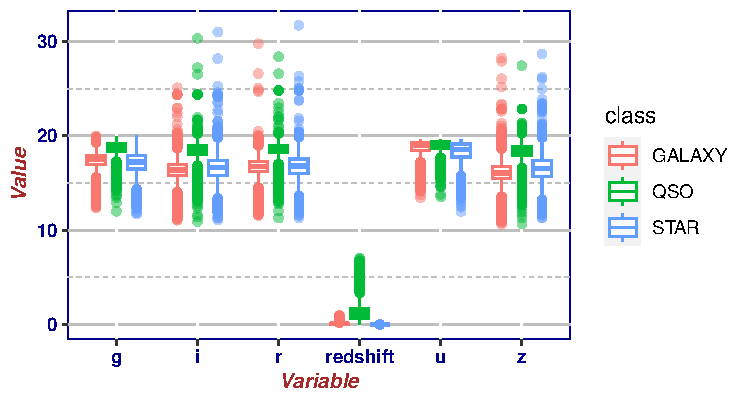
\includegraphics{final_report_files/figure-latex/boxplot-1.pdf}
\caption{\label{fig:boxplot}Boxplot}
\end{figure}

Then, Figure \ref{fig:corr} gives the correlationship between variables in the metadata. We can see that \textbf{redshift} has strong correlationship with the class of the object. Also, the filter variables (\textbf{u}, \textbf{g}, \textbf{r}, \textbf{i}, \textbf{z}) are correlated with each other.

\begin{figure}
\centering
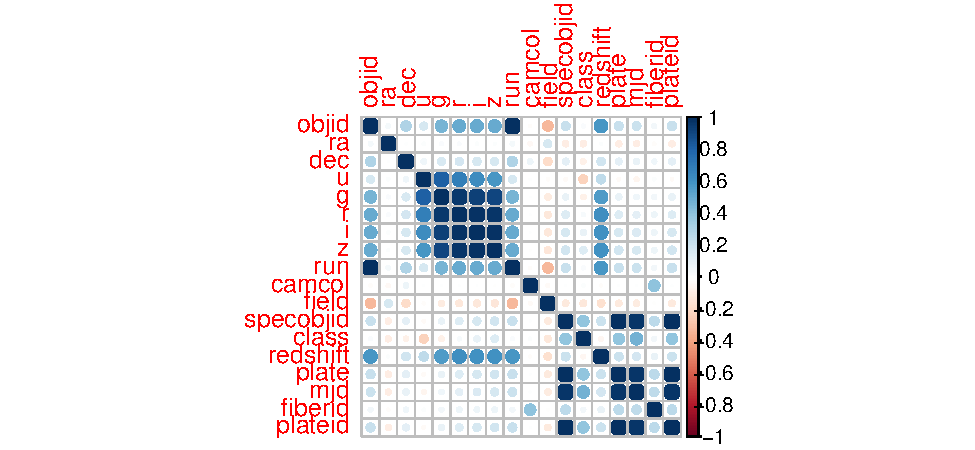
\includegraphics{final_report_files/figure-latex/corr-1.pdf}
\caption{\label{fig:corr}Correlation}
\end{figure}

Next, we will check and deal with missing values in the dataset. For images of the celestial objects, there is no missing value. For images of the spectrum, we have 14115 images that are unreadable. Considering that they are hard to impute, we just ignore them and conduct the analysis on the spectrum based on the rest of the images. For the metadata, there are 1 missing value for \textbf{i} and 3 for \textbf{z}. We use regression imputation with filter variables to impute the missing values as they are correlated with each other and quite scattered.

\hypertarget{methods}{%
\section{Methods}\label{methods}}

For our three types of data, we intend to use three seperate methods to build three different classification models. Then, we plan to use a voting classifier to combine three models and give our final model. In this section, we will give brief introduction to the methods that we have used.

\hypertarget{knn}{%
\subsection{kNN}\label{knn}}

The k-Nearest Neighbors (kNN) algorithm is a simple, but powerful machine learning technique that can be used for classification. At its core, kNN makes predictions about the classification of a data point based on the majority vote or average of its \emph{k} nearest neighbors. With cross validation, we eventually selected \(k = 3\).

\hypertarget{decision-tree}{%
\subsection{Decision Tree}\label{decision-tree}}

A Decision Tree is a machine learning algorithm that can be used for classification. It models decisions and their possible consequences as a tree-like structure, making it intuitive and easy to visualize. The decision-making process starts at the root node and splits the data on the feature that results in the most significant information gain (IG) or the greatest reduction in impurity (such as Gini impurity or entropy). The process continues recursively, creating decision nodes and leaf nodes. Decision nodes ask a question and branch based on the answers to those questions, leading to further splits or to leaf nodes. These nodes represent the outcome. With cross validation and consideration on the complexity of the tree, we set the maximum depth as 4, and use Gini impurity to prune the tree.

\hypertarget{logistic-regression}{%
\subsection{Logistic Regression}\label{logistic-regression}}

Multinomial logistic regression, extends the traditional logistic regression model to handle cases where the target variable categories are more than two. Unlike binary logistic regression, which uses one binary predictor per class, multi-class logistic regression models the probabilities of the multiple classes using a softmax function, which generalizes the logistic function for multi-class problems:

\[
P(Y_i = k) = \frac{e^{\beta_k \cdot X_i}}{\sum_{j = 1}^3 e^{\beta_j \cdot X_i}}, i = 0, 1, 2.
\]

With cross validation, we have selected the hyperparameters as follows: Regularization: L2, \(C = 1\), where the value of \(C\) gives the strength of regularization.

\hypertarget{cnn}{%
\subsection{CNN}\label{cnn}}

Before we get into complex Neural Networks, we firstly try to use a simple CNN to test the performance of NN in this problem. This CNN is quite shallow (337k parameters) with two convolutional layers and a maxpooling in between, followed by three fully connected layers. The structure can be seen in Figure \ref{fig:cnn}. The competitor is VGG16 which is a much deeper NN with 13 convoluntional layers and 3 fully connected layers (138 million parameters).

\hypertarget{voting-classifier}{%
\subsection{Voting Classifier}\label{voting-classifier}}

We try to use two types of voting methods, soft voting and weighted hard voting. Their strategy are slightly different but the idea is similar: to combine the output of several model together to generate a more accurate one.

Suppose we have models \(\{C_1,\cdots C_n\}\), for a given input \(x\). Each model can have a prediction: \(y^i_{pred}|x=(y_1,y_2,y_3)\), where one of \(y_j\) is 1, indicating the predicted class is \(j\), while others are 0. Or a predicting probability: \(P_i(y_j | x)\) which is the predicting probability for x belong to class \(j\) for \(i_{th}\) model.

For kNN and Tree model, their prediction and predicting probability are the same which means their predicting probability is one for predicting class. For soft voting, the prediction is made by average predicting probability of all candidate models and prediction of the voting model is the class with largest predicting probability. The probabilities for voting classifier given input \(x\) is \(P(y_j | x) = \frac{1}{m} \sum_{i=1}^m P_i(y_j | x)\). So the prediction is \(p(x) = \arg \max_{y_j} P(y_j | x)\) where \(m\) is the number of models.

For weighted hard voting, the prediction is made by sum of weighted voting for each class for all the candidate models and prediction of the voting model is the class with largest number of weighted voting. For a given input, \(C_i\) has a predict \(y^{i}|x:~y^{i}_{k=j}=1, ~y^{i}_{k\neq j}=0\) and the prediction for weighted hard voting is \(y_{pred}=\sum_i w_i\cdot y^{i}|x\). So the predict class is \(argmax_j~y_{pred}\).

\hypertarget{results}{%
\section{Results}\label{results}}

\hypertarget{metadata}{%
\subsection{Metadata}\label{metadata}}

For metadata, we have trained three models: kNN, Decision Tree and Logistic Regression.

For the Decision Tree model, the result is shown in Figure \ref{fig:res_dt}. For instance, if the scaled \textbf{redshift} is less or equal than -0.626, scaled \textbf{g} is less or equal than 1.938, then the object should be classified as quasar.

For Logistic Regression model, the result is shown in Table \ref{tab:lr}. The value of intercepts indicate the log odds of being in the respective class when all the predictor values are zero. Each coefficient for the predictors represents the change in the log odds of being in the respective class for a one-unit change in the predictor variable, holding all other predictors constant.

Figure \ref{fig:cm-metadata} gives the confusion matrices for all three models. Combining the evaluations shown in Table \ref{tab:eval} for those three models, we can see a success in building models through the numerical data. By using several indexes and the red shift, our simple models reach more than 96\% accuracy on validation data.

\hypertarget{image-of-celestial-objects}{%
\subsection{Image of Celestial Objects}\label{image-of-celestial-objects}}

The results of this simple CNN is quite good. The cross entropy loss drop quickly after 10k iterations and get stable around 0.27. And the robustness can also be seen on its 90.2\% (SGD), 91.8\% (Adam) average accuracy after 10 epochs training on validation data. Which actually discourages us to apply deeper NN which is quite time and energy consuming. The training took 20 min and the cross entropy loss is under 0.2 after 3 epochs training and stable at 0.18. On the validation data set, VGG has 94.23\% which is better than our simple CNN. However this high accuracy not only consume lot of time but also make it more difficult to improve the performance through the combination of models. Detailed comparison is in Table \ref{tab:cnn-comp} and Figure \ref{fig:loss-cnns}. With these facts, we plan to modify the simple CNN a little without changing its main structure, and use this simple CNN to build up a final model which is expected to have similar performance as VGG16 while consume less time.

The accuracy of CNN of images 91.73\%, CNN of spectrum is 88.91\%. The confusion matrix (Figure \ref{fig:cm-cnn}) shows that CNN classified star (class 2) better than the other celestial objects.

\hypertarget{image-of-spectrum}{%
\subsection{Image of Spectrum}\label{image-of-spectrum}}

The performance of SimpleCNN on spectrum image classification is also very good. We are able to get 0.021 cross entropy loss which is 99.14\% accuracy on validation data set without missing (unreadable) images after 1467 seconds training (Figure \ref{fig:loss-simp-cnn}). And if we include missing value for which the CNN randomly guess a class, the accuracy is 88.91\%.

\hypertarget{voting-classifier-1}{%
\subsection{Voting Classifier}\label{voting-classifier-1}}

If we use voting strategy for only metadata model or CNN, we see a small improve of accuracy on both of them. For metadata models. the soft voting has 97.75\%, weighted hard voting has 97.55\% on validation data set which is better than KNN (96.80\%), Tree model (97.44\%) and Logistic Regression (97.00\%). For CNN models, soft voting: 97.71\%, weighted hard voting: 91.55\% are also better than CNN celestial: 91.73\% and CNN spectrum 88.91\%.

The accuracy of voting classifiers are higher than any single model if we combine metadata models and CNN models together: Soft Voting:98.97\%, Weighted Hard Voting: 98.63\%. From the confusion matrix (Figure \ref{fig:cm-vc}) we can see that both of them classify star (class 2) perfectly followed by Galaxy (class 0) and Quasar (class 1). The detailed model evaluation indexes are shown in Table \ref{tab:eval}

\hypertarget{conclusions}{%
\section{Conclusions}\label{conclusions}}

The voting classifier can improve the accuracy by choosing the best predict class from all the models. And it is more robust for missing data and outliers. From Table 4 we can see that across all evaluation index, soft voting performs better than weighted hard voting. Moreover, for most of the classes, our voting model performs better than single model except for Galaxy and Quasar of image of spectrum data. CNN does a better job for these two class but much worse for Star.
However, the price for better performance is more data used and more model trained. Although we use as simple model as possible for this job, the training and combining is also much more complicated for soft voting and weighted hard voting. In addition, the data we use is in a very good quality and quite sufficient for training a well performed model which is not so common in real situation. The corrupt or insufficient data may affect the accuracy of single models as well as voting classifiers.

According to these facts, our future work may focus on using less models with better voting strategies and using less data with worse data quality to test them.

\newpage

\hypertarget{references}{%
\section{References}\label{references}}

\hypertarget{refs}{}
\begin{CSLReferences}{1}{0}
\leavevmode\vadjust pre{\hypertarget{ref-ref1}{}}%
Gao, Jialin, Jianyu Chen, Jiaqi Wei, Bin Jiang, and A-Li Luo. 2023. {``Deep Multimodal Networks for m-Type Star Classification with Paired Spectrum and Photometric Image.''} \emph{Publications of the Astronomical Society of the Pacific} 135 (May): 044503. \url{https://doi.org/10.1088/1538-3873/acc7ca}.

\end{CSLReferences}

\bibliographystyle{unsrt}
\bibliography{references}

\newpage

\hypertarget{appendix}{%
\section{Appendix}\label{appendix}}

\hypertarget{figures}{%
\subsection{Figures}\label{figures}}

\begin{figure}
\centering
\begin{minipage}{0.45\textwidth}
\centering
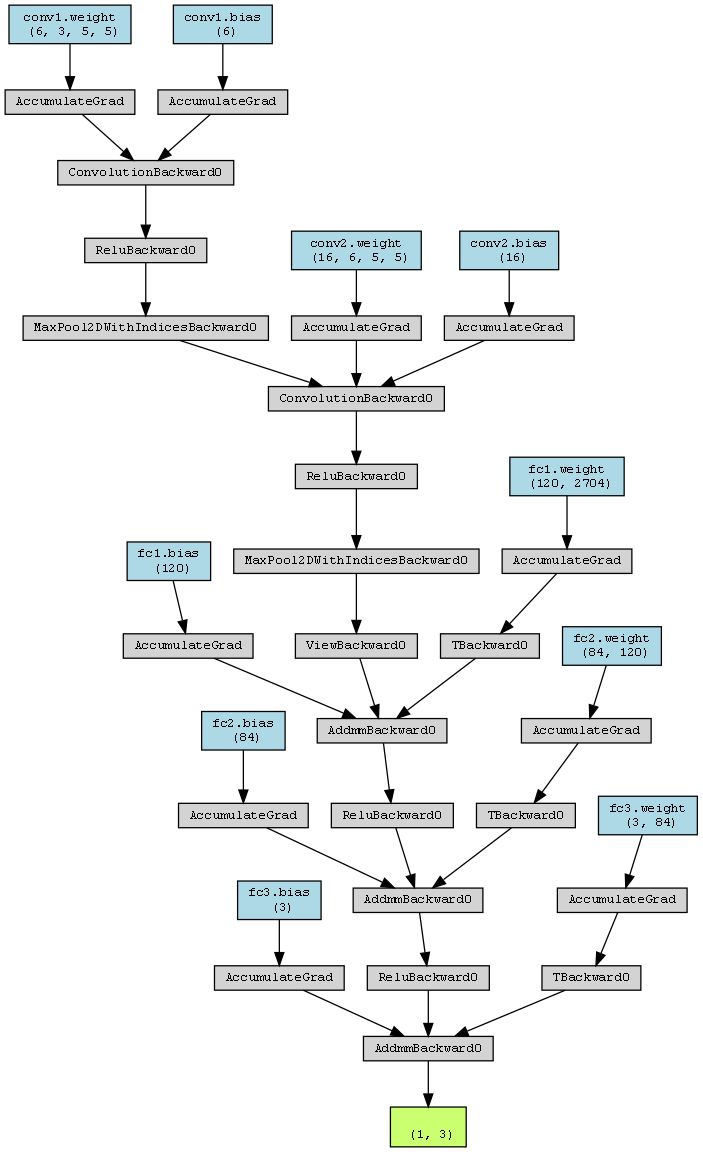
\includegraphics[width=\linewidth]{./data/simple_cnn_visualization.png}
\caption{Structure of CNN}
\label{fig:cnn}
\end{minipage}
\end{figure}

\begin{figure}
\centering
\begin{minipage}{\textwidth}
\centering
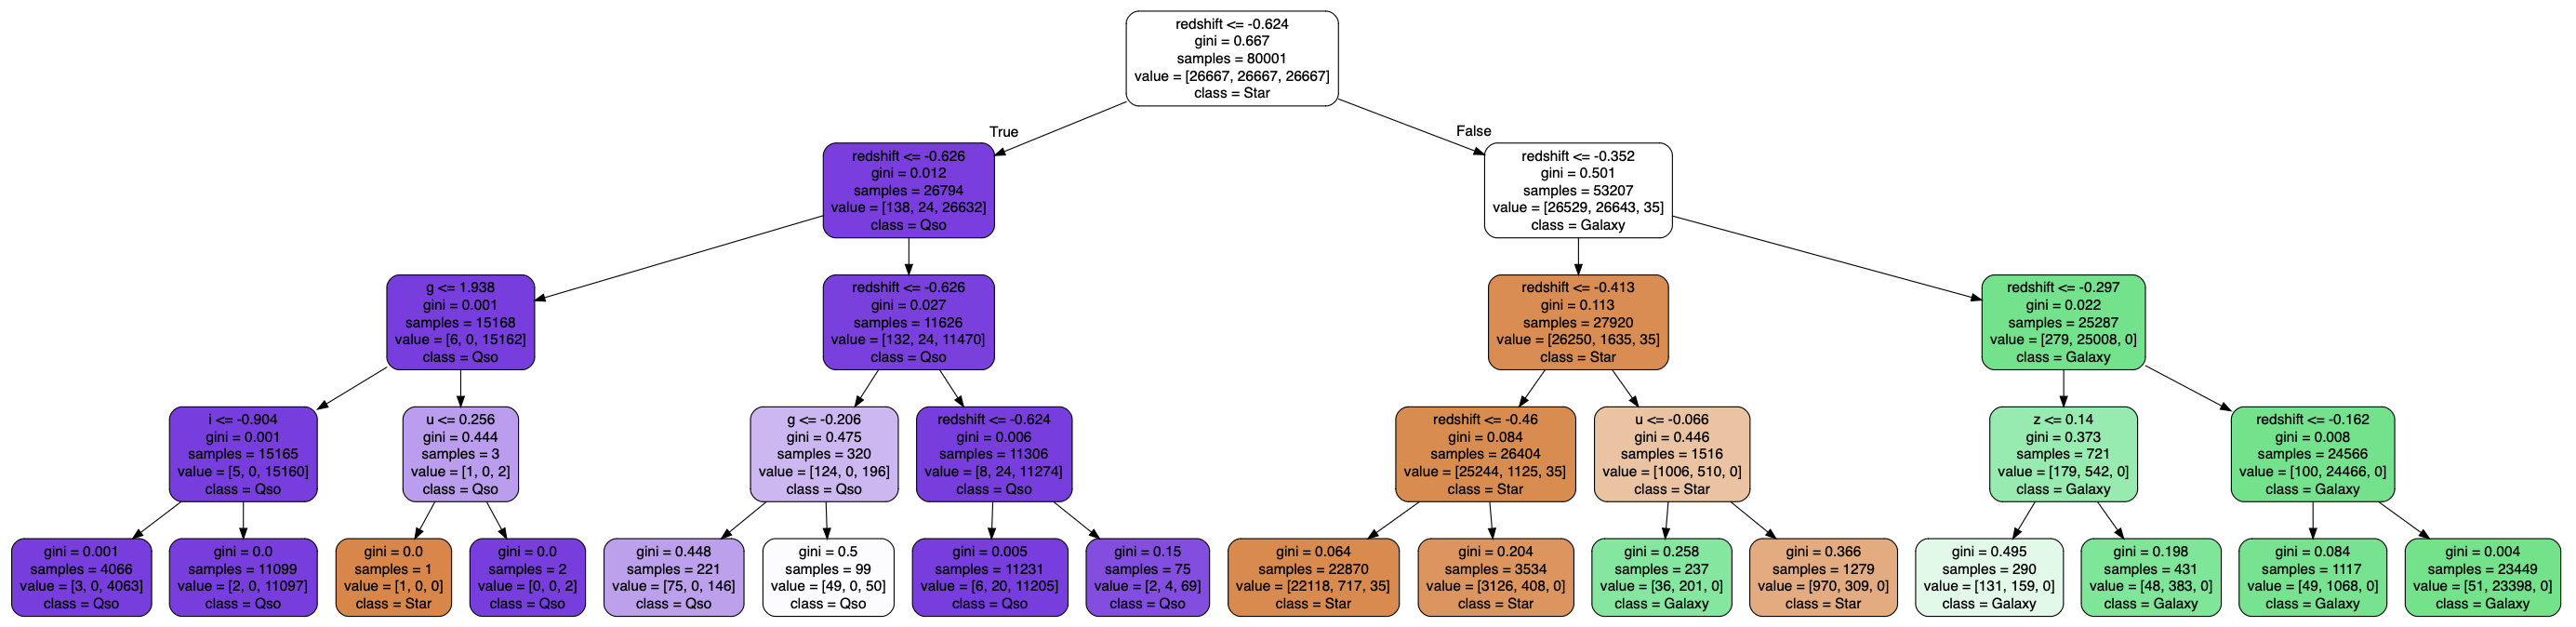
\includegraphics[width=\linewidth]{./images/decision_tree.png}
\caption{Result of Decision Tree}
\label{fig:res_dt}
\end{minipage}
\end{figure}

\begin{figure}
\centering
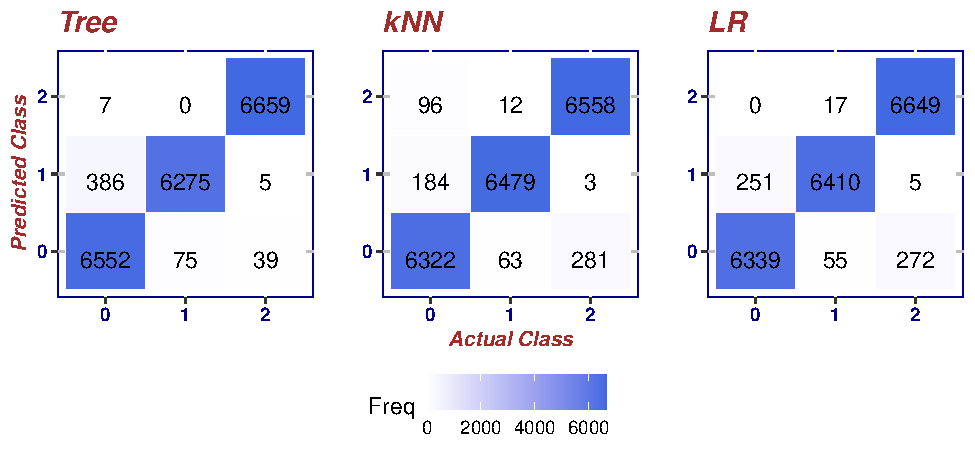
\includegraphics{final_report_files/figure-latex/cm-metadata-1.pdf}
\caption{\label{fig:cm-metadata}Confusion Matrices of Metadata Models}
\end{figure}

\begin{figure}
\centering
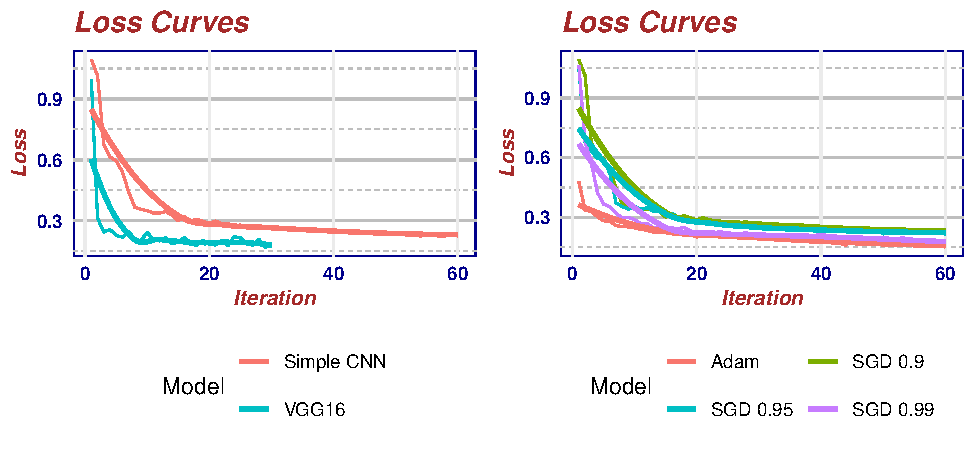
\includegraphics{final_report_files/figure-latex/loss-cnns-1.pdf}
\caption{\label{fig:loss-cnns}Loss Curve Plot for Different CNN}
\end{figure}

\begin{figure}
\centering
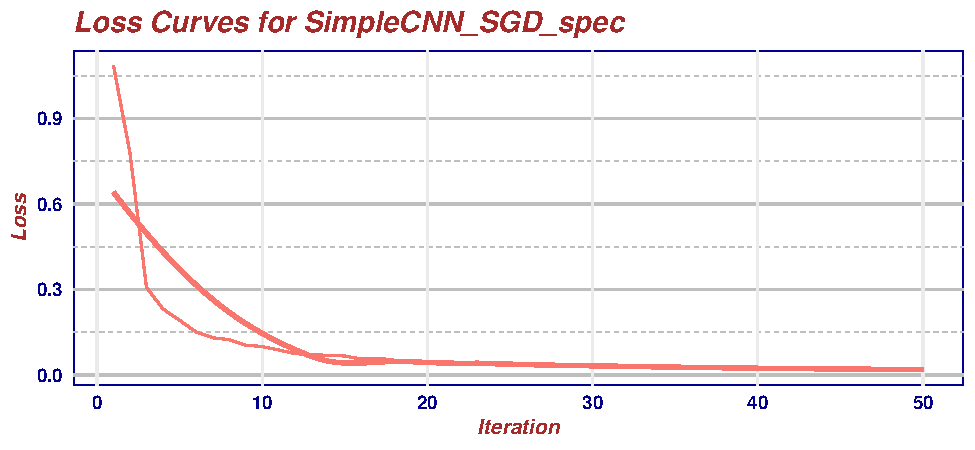
\includegraphics{final_report_files/figure-latex/loss-simp-cnn-1.pdf}
\caption{\label{fig:loss-simp-cnn}Loss Curve}
\end{figure}

\begin{figure}
\centering
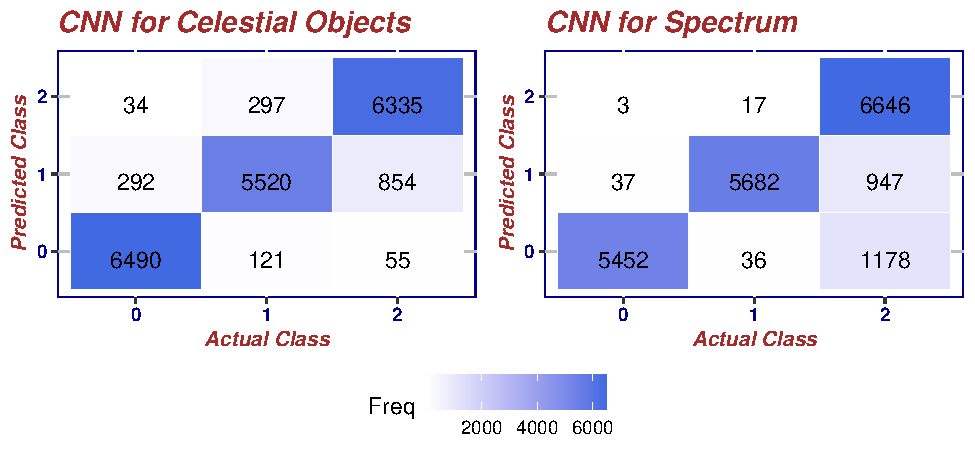
\includegraphics{final_report_files/figure-latex/cm-cnn-1.pdf}
\caption{\label{fig:cm-cnn}Confusion Matrices of CNN Models}
\end{figure}

\begin{figure}
\centering
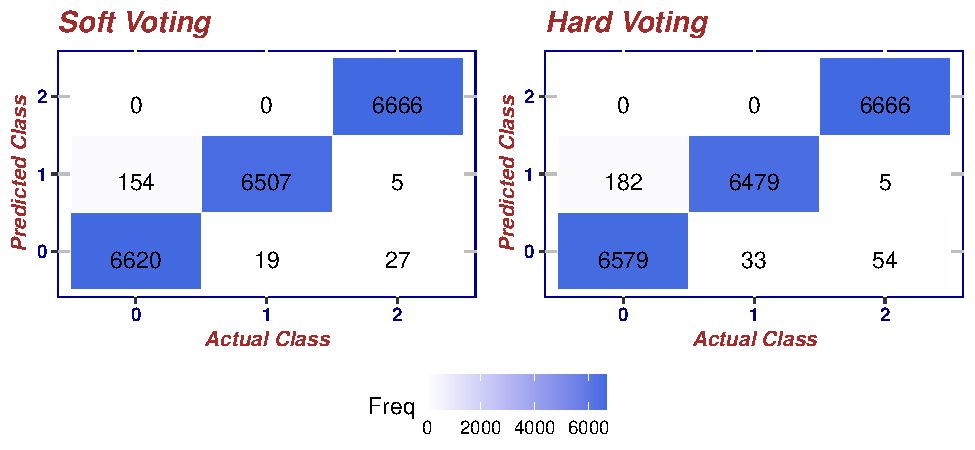
\includegraphics{final_report_files/figure-latex/cm-vc-1.pdf}
\caption{\label{fig:cm-vc}Confusion Matrices of Voting Classifier}
\end{figure}

\quad

\newpage

\hypertarget{tables}{%
\subsection{Tables}\label{tables}}

\begin{table}[H]
\centering
\caption{Metadata of the celestial objects}
\label{tab:metadata}
\centering
\begin{tabular}[t]{ll}
\toprule
Variables & Explanations\\
\midrule
objid & Object Identifier\\
ra & Right Ascension angle (at J2000 epoch)\\
dec & Declination angle (at J2000 epoch)\\
u & Ultraviolet filter\\
g & Green filter\\
\addlinespace
r & Red filter\\
i & Near Infrared filter\\
z & Infrared filter\\
run & Run Number\\
rerun & Rerun Number\\
\addlinespace
camcol & Camera column\\
field & Field number\\
specobjid & Unique ID used for optical spectroscopic objects\\
class & Object class\\
redshift & Redshift value based on the increase in wavelength\\
\addlinespace
plate & Plate\\
mjd & Modified Julian Date\\
fiberid & fiber ID\\
plateid & Plate ID\\
\bottomrule
\end{tabular}
\end{table}

\begin{table}[H]
\centering
\caption{Coefficients of Logistic Regression}
\label{tab:lr}
\centering
\begin{tabular}[t]{lrrrrrrr}
\toprule
  & Intercept & u & g & r & i & z & redshift\\
\midrule
Galaxy & 15.10 & 1.11 & -1.70 & -0.15 & 0.61 & -0.02 & 23.36\\
Qso & 16.81 & -2.88 & 5.21 & 0.80 & -1.22 & -2.14 & 32.51\\
Star & -31.91 & 1.77 & -3.51 & -0.64 & 0.61 & 2.16 & -55.86\\
\bottomrule
\end{tabular}
\end{table}

\begin{table}[H]
\centering
\caption{CNN Model Comparison}
\label{tab:cnn-comp}
\centering
\begin{tabular}[t]{lll}
\toprule
Name & Accuracy & Training.Time\\
\midrule
SimpleCNN & 91.68\% & 635 s\\
VGG16 & 94.11\% & 1281 s\\
Res18 & 94.89\% & 1324 s\\
\bottomrule
\end{tabular}
\end{table}

\begin{table}[H]
\centering
\caption{Simple CNN Tuning Comparison}
\label{tab:simple-cnn}
\centering
\begin{tabular}[t]{lll}
\toprule
Optimizer & Accuray & Training.Time\\
\midrule
SGD\_mom0.9 & 91.68\% & 458 s\\
SGD\_mom0.95 & 92.84\% & 463 s\\
SGD\_mom0.99 & 93.78\% & 462 s\\
Adam & 93.91\% & 463 s\\
\bottomrule
\end{tabular}
\end{table}

\begin{table}[H]
\centering
\caption{Evaluation of Models}
\label{tab:eval}
\centering
\begin{tabular}[t]{ccccccccc}
\toprule
Data &  & M & M & M & IC & IS & M+IC+IS & M+IC+IS\\
\midrule
Model &  & kNN & DT & LR & CNN & CNN & SVC & HVC\\
\midrule
Accuracy &  & 0.968 & 0.9744 & 0.97 & 0.9173 & 0.8891 & 0.9897 & 0.9863\\
\addlinespace
& Galaxy & 0.9576 & 0.9434 & 0.9619 & 0.9522 & 0.9927 & 0.9773 & 0.9731\\
Precision & Qso & 0.9886 & 0.9882 & 0.9889 & 0.9296 & 0.9908 & 0.9971 & 0.9949\\
& Star & 0.9585 & 0.9934 & 0.96 & 0.8745 & 0.7577 & 0.9952 & 0.9912\\
\addlinespace
& Galaxy & 0.9484 & 0.9829 & 0.9509 & 0.9736 & 0.8179 & 0.9931 & 0.9869\\
Recall & Qso & 0.9719 & 0.9413 & 0.9616 & 0.8281 & 0.8524 & 0.9761 & 0.9719\\
& Star & 0.9838 & 0.9989 & 0.9974 & 0.9503 & 0.997 & 1 & 1\\
\addlinespace
& Galaxy & 0.953 & 0.9628 & 0.9564 & 0.9628 & 0.8969 & 0.9851 & 0.98\\
F1 & Qso & 0.9802 & 0.9642 & 0.9751 & 0.8759 & 0.9164 & 0.9865 & 0.9833\\
& Star & 0.971 & 0.9962 & 0.9784 & 0.9109 & 0.861 & 0.9976 & 0.9956\\
\bottomrule
\multicolumn{9}{l}{\rule{0pt}{1em}\textit{Note: }}\\
\multicolumn{9}{l}{\rule{0pt}{1em}M: Metadata. IC: Image of Celestial Objects. IS: Image of Spectrum.}\\
\end{tabular}
\end{table}

\end{document}
